\chapter{Auswertung}

\section{Kalibrierung}
Um den Totalreflexionswinkel zu bestimmen haben wir f�r verschiedene Wellenl�ngen von 500nm - 600nm 
einen gro�en Winkel zwischen 0 und 90 Grad bzgl des einfallenden Lichtstrahles abgefahren und die Reflexivit�t
des Glasprismas unter diesem Winkel gemessen.

Wir erwarten einen stufenf�rmigen Verlauf wobei die Reflexivit�t bei 0 anf�ngt, an dem Totalreflexionswinkel
auf 1 springt und bis 90 Grad weiterverl�uft. 

\begin{equation}
 \theta_{tot}=arcsin{\sqrt{\frac{\eps_{Luft}}{\eps_{Glas}(\lambda)}}}
\end{equation}

Dies ist eine idealisierte Betrachtungsweise. Wir werden im Experiment eine stetige Kurve an der Totalreflexionsstelle sehen
und versuchen f�r jeden Messdurchlauf diese Stelle mit 2 Geraden anzufitten.

\begin{figure}[h]
    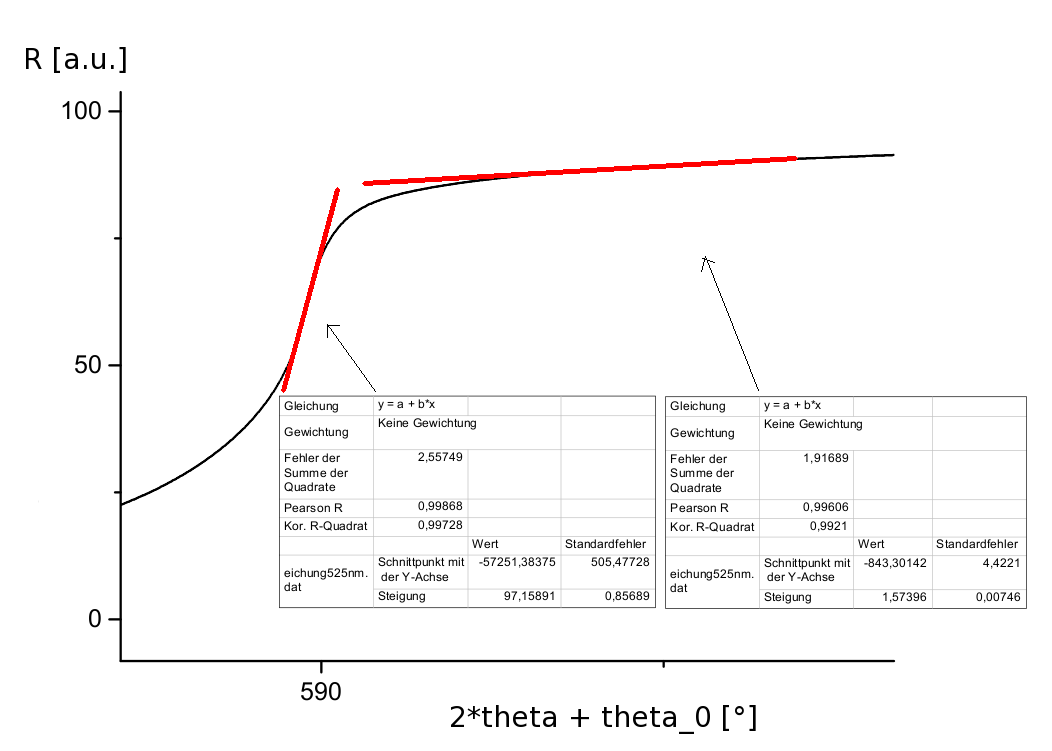
\includegraphics[width=1\textwidth]{linreg-totref-525nm.png}
	\caption{Gemessene Reflektivit�t $R$ in Abh�ngigkeit der zu kalibrierenden Winkelangabe
				des Rotationstisches $2\theta+\theta_0$. In Rot die linearen Regressionen
				zur Bestimmung des Totalreflexionswinkels.}
	\label{fig:linreg}
\end{figure}


Wir beziehen uns hier auf \eqref{eq:r012}